% GNUPLOT: LaTeX picture with Postscript
\begingroup
  \makeatletter
  \providecommand\color[2][]{%
    \GenericError{(gnuplot) \space\space\space\@spaces}{%
      Package color not loaded in conjunction with
      terminal option `colourtext'%
    }{See the gnuplot documentation for explanation.%
    }{Either use 'blacktext' in gnuplot or load the package
      color.sty in LaTeX.}%
    \renewcommand\color[2][]{}%
  }%
  \providecommand\includegraphics[2][]{%
    \GenericError{(gnuplot) \space\space\space\@spaces}{%
      Package graphicx or graphics not loaded%
    }{See the gnuplot documentation for explanation.%
    }{The gnuplot epslatex terminal needs graphicx.sty or graphics.sty.}%
    \renewcommand\includegraphics[2][]{}%
  }%
  \providecommand\rotatebox[2]{#2}%
  \@ifundefined{ifGPcolor}{%
    \newif\ifGPcolor
    \GPcolortrue
  }{}%
  \@ifundefined{ifGPblacktext}{%
    \newif\ifGPblacktext
    \GPblacktextfalse
  }{}%
  % define a \g@addto@macro without @ in the name:
  \let\gplgaddtomacro\g@addto@macro
  % define empty templates for all commands taking text:
  \gdef\gplbacktext{}%
  \gdef\gplfronttext{}%
  \makeatother
  \ifGPblacktext
    % no textcolor at all
    \def\colorrgb#1{}%
    \def\colorgray#1{}%
  \else
    % gray or color?
    \ifGPcolor
      \def\colorrgb#1{\color[rgb]{#1}}%
      \def\colorgray#1{\color[gray]{#1}}%
      \expandafter\def\csname LTw\endcsname{\color{white}}%
      \expandafter\def\csname LTb\endcsname{\color{black}}%
      \expandafter\def\csname LTa\endcsname{\color{black}}%
      \expandafter\def\csname LT0\endcsname{\color[rgb]{1,0,0}}%
      \expandafter\def\csname LT1\endcsname{\color[rgb]{0,1,0}}%
      \expandafter\def\csname LT2\endcsname{\color[rgb]{0,0,1}}%
      \expandafter\def\csname LT3\endcsname{\color[rgb]{1,0,1}}%
      \expandafter\def\csname LT4\endcsname{\color[rgb]{0,1,1}}%
      \expandafter\def\csname LT5\endcsname{\color[rgb]{1,1,0}}%
      \expandafter\def\csname LT6\endcsname{\color[rgb]{0,0,0}}%
      \expandafter\def\csname LT7\endcsname{\color[rgb]{1,0.3,0}}%
      \expandafter\def\csname LT8\endcsname{\color[rgb]{0.5,0.5,0.5}}%
    \else
      % gray
      \def\colorrgb#1{\color{black}}%
      \def\colorgray#1{\color[gray]{#1}}%
      \expandafter\def\csname LTw\endcsname{\color{white}}%
      \expandafter\def\csname LTb\endcsname{\color{black}}%
      \expandafter\def\csname LTa\endcsname{\color{black}}%
      \expandafter\def\csname LT0\endcsname{\color{black}}%
      \expandafter\def\csname LT1\endcsname{\color{black}}%
      \expandafter\def\csname LT2\endcsname{\color{black}}%
      \expandafter\def\csname LT3\endcsname{\color{black}}%
      \expandafter\def\csname LT4\endcsname{\color{black}}%
      \expandafter\def\csname LT5\endcsname{\color{black}}%
      \expandafter\def\csname LT6\endcsname{\color{black}}%
      \expandafter\def\csname LT7\endcsname{\color{black}}%
      \expandafter\def\csname LT8\endcsname{\color{black}}%
    \fi
  \fi
    \setlength{\unitlength}{0.0500bp}%
    \ifx\gptboxheight\undefined%
      \newlength{\gptboxheight}%
      \newlength{\gptboxwidth}%
      \newsavebox{\gptboxtext}%
    \fi%
    \setlength{\fboxrule}{0.5pt}%
    \setlength{\fboxsep}{1pt}%
\begin{picture}(7580.00,7360.00)%
    \gplgaddtomacro\gplbacktext{%
      \csname LTb\endcsname%%
      \put(578,5229){\makebox(0,0)[r]{\strut{}\tiny -0.5}}%
      \csname LTb\endcsname%%
      \put(578,5699){\makebox(0,0)[r]{\strut{}\tiny -0.25}}%
      \csname LTb\endcsname%%
      \put(578,6169){\makebox(0,0)[r]{\strut{}\tiny 0}}%
      \csname LTb\endcsname%%
      \put(578,6638){\makebox(0,0)[r]{\strut{}\tiny 0.25}}%
      \csname LTb\endcsname%%
      \put(578,7108){\makebox(0,0)[r]{\strut{}\tiny 0.5}}%
      \csname LTb\endcsname%%
      \put(646,5105){\makebox(0,0){\strut{}\tiny -0.5}}%
      \csname LTb\endcsname%%
      \put(1116,5105){\makebox(0,0){\strut{}\tiny -0.25}}%
      \csname LTb\endcsname%%
      \put(1585,5105){\makebox(0,0){\strut{}\tiny 0}}%
      \csname LTb\endcsname%%
      \put(2055,5105){\makebox(0,0){\strut{}\tiny 0.25}}%
      \csname LTb\endcsname%%
      \put(2524,5105){\makebox(0,0){\strut{}\tiny 0.5}}%
      \colorrgb{1.00,0.00,0.00}%%
      \put(76,6133){\makebox(0,0)[l]{\strut{}O}}%
      \colorrgb{0.00,0.00,1.00}%%
      \put(76,3827){\makebox(0,0)[l]{\strut{}Li}}%
      \colorrgb{0.00,0.32,0.19}%%
      \put(76,1374){\makebox(0,0)[l]{\strut{}Cl}}%
    }%
    \gplgaddtomacro\gplfronttext{%
      \csname LTb\endcsname%%
      \put(1585,7294){\makebox(0,0){\strut{}1 mol/L}}%
    }%
    \gplgaddtomacro\gplbacktext{%
      \csname LTb\endcsname%%
      \put(2915,5229){\makebox(0,0)[r]{\strut{}\tiny -0.5}}%
      \csname LTb\endcsname%%
      \put(2915,5699){\makebox(0,0)[r]{\strut{}\tiny -0.25}}%
      \csname LTb\endcsname%%
      \put(2915,6169){\makebox(0,0)[r]{\strut{}\tiny 0}}%
      \csname LTb\endcsname%%
      \put(2915,6638){\makebox(0,0)[r]{\strut{}\tiny 0.25}}%
      \csname LTb\endcsname%%
      \put(2915,7108){\makebox(0,0)[r]{\strut{}\tiny 0.5}}%
      \csname LTb\endcsname%%
      \put(2983,5105){\makebox(0,0){\strut{}\tiny -0.5}}%
      \csname LTb\endcsname%%
      \put(3453,5105){\makebox(0,0){\strut{}\tiny -0.25}}%
      \csname LTb\endcsname%%
      \put(3922,5105){\makebox(0,0){\strut{}\tiny 0}}%
      \csname LTb\endcsname%%
      \put(4392,5105){\makebox(0,0){\strut{}\tiny 0.25}}%
      \csname LTb\endcsname%%
      \put(4861,5105){\makebox(0,0){\strut{}\tiny 0.5}}%
      \colorrgb{1.00,0.00,0.00}%%
      \put(76,6133){\makebox(0,0)[l]{\strut{}O}}%
      \colorrgb{0.00,0.00,1.00}%%
      \put(76,3827){\makebox(0,0)[l]{\strut{}Li}}%
      \colorrgb{0.00,0.32,0.19}%%
      \put(76,1374){\makebox(0,0)[l]{\strut{}Cl}}%
    }%
    \gplgaddtomacro\gplfronttext{%
      \csname LTb\endcsname%%
      \put(3922,7294){\makebox(0,0){\strut{}10 mol/L}}%
    }%
    \gplgaddtomacro\gplbacktext{%
      \csname LTb\endcsname%%
      \put(5252,5229){\makebox(0,0)[r]{\strut{}\tiny -0.5}}%
      \csname LTb\endcsname%%
      \put(5252,5699){\makebox(0,0)[r]{\strut{}\tiny -0.25}}%
      \csname LTb\endcsname%%
      \put(5252,6169){\makebox(0,0)[r]{\strut{}\tiny 0}}%
      \csname LTb\endcsname%%
      \put(5252,6638){\makebox(0,0)[r]{\strut{}\tiny 0.25}}%
      \csname LTb\endcsname%%
      \put(5252,7108){\makebox(0,0)[r]{\strut{}\tiny 0.5}}%
      \csname LTb\endcsname%%
      \put(5320,5105){\makebox(0,0){\strut{}\tiny -0.5}}%
      \csname LTb\endcsname%%
      \put(5790,5105){\makebox(0,0){\strut{}\tiny -0.25}}%
      \csname LTb\endcsname%%
      \put(6259,5105){\makebox(0,0){\strut{}\tiny 0}}%
      \csname LTb\endcsname%%
      \put(6729,5105){\makebox(0,0){\strut{}\tiny 0.25}}%
      \csname LTb\endcsname%%
      \put(7198,5105){\makebox(0,0){\strut{}\tiny 0.5}}%
      \colorrgb{1.00,0.00,0.00}%%
      \put(76,6133){\makebox(0,0)[l]{\strut{}O}}%
      \colorrgb{0.00,0.00,1.00}%%
      \put(76,3827){\makebox(0,0)[l]{\strut{}Li}}%
      \colorrgb{0.00,0.32,0.19}%%
      \put(76,1374){\makebox(0,0)[l]{\strut{}Cl}}%
    }%
    \gplgaddtomacro\gplfronttext{%
      \csname LTb\endcsname%%
      \put(6259,7294){\makebox(0,0){\strut{}20 mol/L}}%
    }%
    \gplgaddtomacro\gplbacktext{%
      \csname LTb\endcsname%%
      \put(578,2900){\makebox(0,0)[r]{\strut{}\tiny -0.5}}%
      \csname LTb\endcsname%%
      \put(578,3370){\makebox(0,0)[r]{\strut{}\tiny -0.25}}%
      \csname LTb\endcsname%%
      \put(578,3840){\makebox(0,0)[r]{\strut{}\tiny 0}}%
      \csname LTb\endcsname%%
      \put(578,4309){\makebox(0,0)[r]{\strut{}\tiny 0.25}}%
      \csname LTb\endcsname%%
      \put(578,4779){\makebox(0,0)[r]{\strut{}\tiny 0.5}}%
      \csname LTb\endcsname%%
      \put(646,2776){\makebox(0,0){\strut{}\tiny -0.5}}%
      \csname LTb\endcsname%%
      \put(1116,2776){\makebox(0,0){\strut{}\tiny -0.25}}%
      \csname LTb\endcsname%%
      \put(1585,2776){\makebox(0,0){\strut{}\tiny 0}}%
      \csname LTb\endcsname%%
      \put(2055,2776){\makebox(0,0){\strut{}\tiny 0.25}}%
      \csname LTb\endcsname%%
      \put(2524,2776){\makebox(0,0){\strut{}\tiny 0.5}}%
      \colorrgb{1.00,0.00,0.00}%%
      \put(76,6133){\makebox(0,0)[l]{\strut{}O}}%
      \colorrgb{0.00,0.00,1.00}%%
      \put(76,3827){\makebox(0,0)[l]{\strut{}Li}}%
      \colorrgb{0.00,0.32,0.19}%%
      \put(76,1374){\makebox(0,0)[l]{\strut{}Cl}}%
    }%
    \gplgaddtomacro\gplfronttext{%
    }%
    \gplgaddtomacro\gplbacktext{%
      \csname LTb\endcsname%%
      \put(2915,2900){\makebox(0,0)[r]{\strut{}\tiny -0.5}}%
      \csname LTb\endcsname%%
      \put(2915,3370){\makebox(0,0)[r]{\strut{}\tiny -0.25}}%
      \csname LTb\endcsname%%
      \put(2915,3840){\makebox(0,0)[r]{\strut{}\tiny 0}}%
      \csname LTb\endcsname%%
      \put(2915,4309){\makebox(0,0)[r]{\strut{}\tiny 0.25}}%
      \csname LTb\endcsname%%
      \put(2915,4779){\makebox(0,0)[r]{\strut{}\tiny 0.5}}%
      \csname LTb\endcsname%%
      \put(2983,2776){\makebox(0,0){\strut{}\tiny -0.5}}%
      \csname LTb\endcsname%%
      \put(3453,2776){\makebox(0,0){\strut{}\tiny -0.25}}%
      \csname LTb\endcsname%%
      \put(3922,2776){\makebox(0,0){\strut{}\tiny 0}}%
      \csname LTb\endcsname%%
      \put(4392,2776){\makebox(0,0){\strut{}\tiny 0.25}}%
      \csname LTb\endcsname%%
      \put(4861,2776){\makebox(0,0){\strut{}\tiny 0.5}}%
      \colorrgb{1.00,0.00,0.00}%%
      \put(76,6133){\makebox(0,0)[l]{\strut{}O}}%
      \colorrgb{0.00,0.00,1.00}%%
      \put(76,3827){\makebox(0,0)[l]{\strut{}Li}}%
      \colorrgb{0.00,0.32,0.19}%%
      \put(76,1374){\makebox(0,0)[l]{\strut{}Cl}}%
    }%
    \gplgaddtomacro\gplfronttext{%
    }%
    \gplgaddtomacro\gplbacktext{%
      \csname LTb\endcsname%%
      \put(5252,2900){\makebox(0,0)[r]{\strut{}\tiny -0.5}}%
      \csname LTb\endcsname%%
      \put(5252,3370){\makebox(0,0)[r]{\strut{}\tiny -0.25}}%
      \csname LTb\endcsname%%
      \put(5252,3840){\makebox(0,0)[r]{\strut{}\tiny 0}}%
      \csname LTb\endcsname%%
      \put(5252,4309){\makebox(0,0)[r]{\strut{}\tiny 0.25}}%
      \csname LTb\endcsname%%
      \put(5252,4779){\makebox(0,0)[r]{\strut{}\tiny 0.5}}%
      \csname LTb\endcsname%%
      \put(5320,2776){\makebox(0,0){\strut{}\tiny -0.5}}%
      \csname LTb\endcsname%%
      \put(5790,2776){\makebox(0,0){\strut{}\tiny -0.25}}%
      \csname LTb\endcsname%%
      \put(6259,2776){\makebox(0,0){\strut{}\tiny 0}}%
      \csname LTb\endcsname%%
      \put(6729,2776){\makebox(0,0){\strut{}\tiny 0.25}}%
      \csname LTb\endcsname%%
      \put(7198,2776){\makebox(0,0){\strut{}\tiny 0.5}}%
      \colorrgb{1.00,0.00,0.00}%%
      \put(76,6133){\makebox(0,0)[l]{\strut{}O}}%
      \colorrgb{0.00,0.00,1.00}%%
      \put(76,3827){\makebox(0,0)[l]{\strut{}Li}}%
      \colorrgb{0.00,0.32,0.19}%%
      \put(76,1374){\makebox(0,0)[l]{\strut{}Cl}}%
    }%
    \gplgaddtomacro\gplfronttext{%
    }%
    \gplgaddtomacro\gplbacktext{%
      \csname LTb\endcsname%%
      \put(578,447){\makebox(0,0)[r]{\strut{}\tiny -0.5}}%
      \csname LTb\endcsname%%
      \put(578,917){\makebox(0,0)[r]{\strut{}\tiny -0.25}}%
      \csname LTb\endcsname%%
      \put(578,1387){\makebox(0,0)[r]{\strut{}\tiny 0}}%
      \csname LTb\endcsname%%
      \put(578,1856){\makebox(0,0)[r]{\strut{}\tiny 0.25}}%
      \csname LTb\endcsname%%
      \put(578,2326){\makebox(0,0)[r]{\strut{}\tiny 0.5}}%
      \csname LTb\endcsname%%
      \put(646,323){\makebox(0,0){\strut{}\tiny -0.5}}%
      \csname LTb\endcsname%%
      \put(1116,323){\makebox(0,0){\strut{}\tiny -0.25}}%
      \csname LTb\endcsname%%
      \put(1585,323){\makebox(0,0){\strut{}\tiny 0}}%
      \csname LTb\endcsname%%
      \put(2055,323){\makebox(0,0){\strut{}\tiny 0.25}}%
      \csname LTb\endcsname%%
      \put(2524,323){\makebox(0,0){\strut{}\tiny 0.5}}%
      \colorrgb{1.00,0.00,0.00}%%
      \put(76,6133){\makebox(0,0)[l]{\strut{}O}}%
      \colorrgb{0.00,0.00,1.00}%%
      \put(76,3827){\makebox(0,0)[l]{\strut{}Li}}%
      \colorrgb{0.00,0.32,0.19}%%
      \put(76,1374){\makebox(0,0)[l]{\strut{}Cl}}%
    }%
    \gplgaddtomacro\gplfronttext{%
    }%
    \gplgaddtomacro\gplbacktext{%
      \csname LTb\endcsname%%
      \put(2915,447){\makebox(0,0)[r]{\strut{}\tiny -0.5}}%
      \csname LTb\endcsname%%
      \put(2915,917){\makebox(0,0)[r]{\strut{}\tiny -0.25}}%
      \csname LTb\endcsname%%
      \put(2915,1387){\makebox(0,0)[r]{\strut{}\tiny 0}}%
      \csname LTb\endcsname%%
      \put(2915,1856){\makebox(0,0)[r]{\strut{}\tiny 0.25}}%
      \csname LTb\endcsname%%
      \put(2915,2326){\makebox(0,0)[r]{\strut{}\tiny 0.5}}%
      \csname LTb\endcsname%%
      \put(2983,323){\makebox(0,0){\strut{}\tiny -0.5}}%
      \csname LTb\endcsname%%
      \put(3453,323){\makebox(0,0){\strut{}\tiny -0.25}}%
      \csname LTb\endcsname%%
      \put(3922,323){\makebox(0,0){\strut{}\tiny 0}}%
      \csname LTb\endcsname%%
      \put(4392,323){\makebox(0,0){\strut{}\tiny 0.25}}%
      \csname LTb\endcsname%%
      \put(4861,323){\makebox(0,0){\strut{}\tiny 0.5}}%
      \colorrgb{1.00,0.00,0.00}%%
      \put(76,6133){\makebox(0,0)[l]{\strut{}O}}%
      \colorrgb{0.00,0.00,1.00}%%
      \put(76,3827){\makebox(0,0)[l]{\strut{}Li}}%
      \colorrgb{0.00,0.32,0.19}%%
      \put(76,1374){\makebox(0,0)[l]{\strut{}Cl}}%
    }%
    \gplgaddtomacro\gplfronttext{%
    }%
    \gplgaddtomacro\gplbacktext{%
      \csname LTb\endcsname%%
      \put(5252,447){\makebox(0,0)[r]{\strut{}\tiny -0.5}}%
      \csname LTb\endcsname%%
      \put(5252,917){\makebox(0,0)[r]{\strut{}\tiny -0.25}}%
      \csname LTb\endcsname%%
      \put(5252,1387){\makebox(0,0)[r]{\strut{}\tiny 0}}%
      \csname LTb\endcsname%%
      \put(5252,1856){\makebox(0,0)[r]{\strut{}\tiny 0.25}}%
      \csname LTb\endcsname%%
      \put(5252,2326){\makebox(0,0)[r]{\strut{}\tiny 0.5}}%
      \csname LTb\endcsname%%
      \put(5320,323){\makebox(0,0){\strut{}\tiny -0.5}}%
      \csname LTb\endcsname%%
      \put(5790,323){\makebox(0,0){\strut{}\tiny -0.25}}%
      \csname LTb\endcsname%%
      \put(6259,323){\makebox(0,0){\strut{}\tiny 0}}%
      \csname LTb\endcsname%%
      \put(6729,323){\makebox(0,0){\strut{}\tiny 0.25}}%
      \csname LTb\endcsname%%
      \put(7198,323){\makebox(0,0){\strut{}\tiny 0.5}}%
      \colorrgb{1.00,0.00,0.00}%%
      \put(76,6133){\makebox(0,0)[l]{\strut{}O}}%
      \colorrgb{0.00,0.00,1.00}%%
      \put(76,3827){\makebox(0,0)[l]{\strut{}Li}}%
      \colorrgb{0.00,0.32,0.19}%%
      \put(76,1374){\makebox(0,0)[l]{\strut{}Cl}}%
    }%
    \gplgaddtomacro\gplfronttext{%
    }%
    \gplbacktext
    \put(0,0){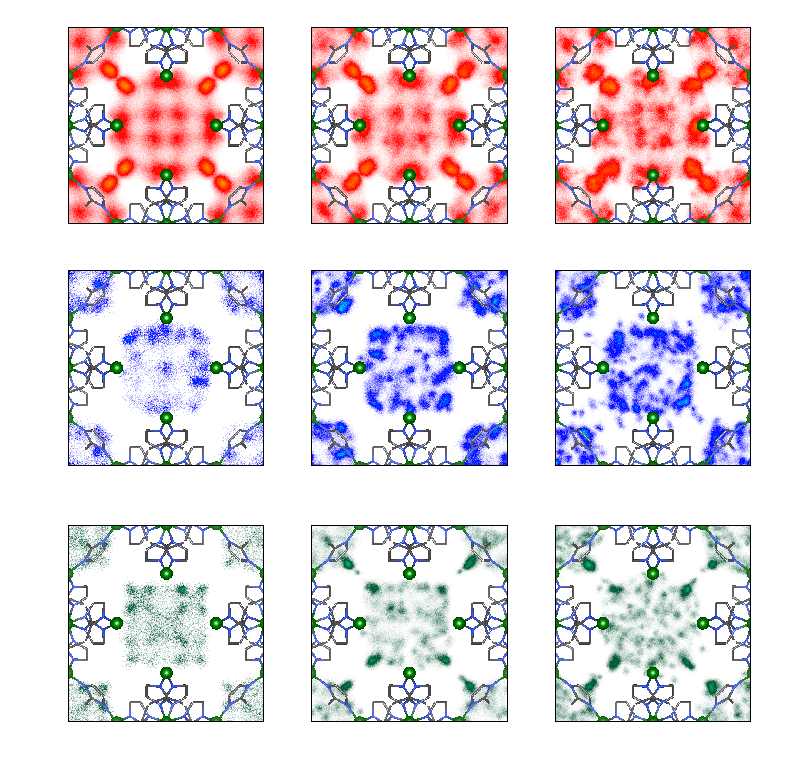
\includegraphics{licl-zif-density}}%
    \gplfronttext
  \end{picture}%
\endgroup
